% Especificaciones del tamaño de letra, tamaño de hoja, márgenes, librerias, etc.
\documentclass[12pt, letterpaper]{article}
\usepackage[english]{babel}
\usepackage{fancyhdr}
\usepackage[utf8]{inputenc}
\usepackage[T1]{fontenc}
\usepackage{amsmath}
\usepackage{graphicx}
\usepackage{subcaption}
\usepackage[hidelinks]{hyperref}
\usepackage{url}
\usepackage{amssymb}
\usepackage{float}
\usepackage[margin=1in]{geometry}
\renewcommand{\baselinestretch}{1.5}

% Enlace Bibliografía
\usepackage{csquotes}
\usepackage[notes,backend=biber]{biblatex-chicago}
\addbibresource{referencias.bib}

% Titulo, autores, fecha.
\title{Homework \#2: Combustors}
\author{Carlos A. Vásquez Castañeda \and 1155057 \and Group 392}
\date{October 2, 2019}
\pagestyle{fancy}
\fancyhf{}
\rhead{Aircraft Elements Design}
\lhead{Homework \#2}
\rfoot{\thepage}


% Inicio del documento
\begin{document}
\maketitle
\section*{Introduction}
The combustor (also known as combustion chamber, burner or flame holder), is where combustion of the air from a jet engine takes place. The turbine of a jet engine needs to draw power from somewhere in order to turn, and so, the combustor is in charge of combining fuel with high pressure air and ignite it in order to produce high temperature gas that will go through the turbine, giving it power, and it will also provide thrust when passed through a nozzle. \autocite{nasacomb}

The design of combustion chambers needs to be given thourough attention, as it plays a crucial role in determining most of the engine's operating characteristics, such as fuel efficiency, levels of emissions and the transient response (the response to changing conditions such as fuel flow and air speed).

\begin{figure}[H]
	\centering
	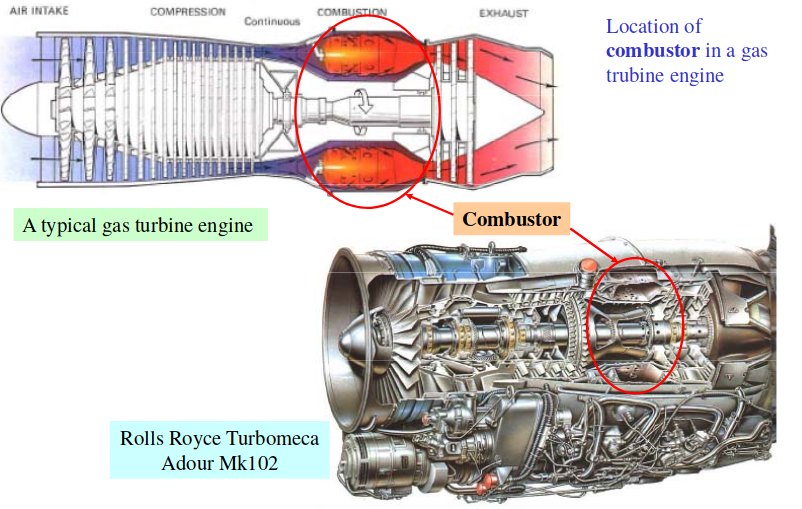
\includegraphics[width=0.4\textwidth]{1.png}
	\caption{Usual location of the combustion chamber.}
\end{figure}

The parts of the combustor are generally portraited as shown below:

\begin{figure}[H]
	\centering
	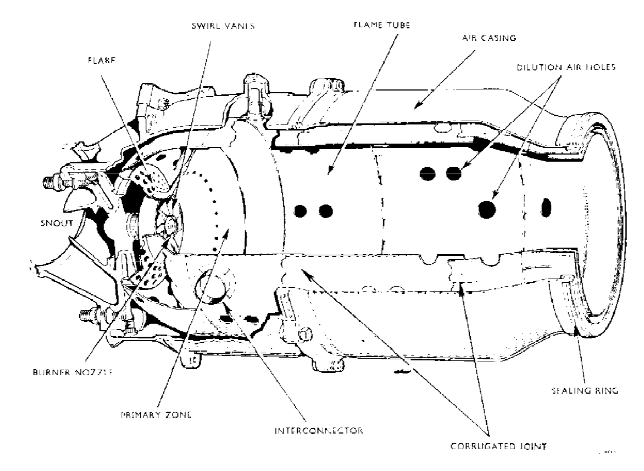
\includegraphics[width=0.7\textwidth]{2.png}
	\caption{Parts of a combustion chamber.}
\end{figure}

Probably the most essential parts of the combustion chamber is the snout, where air from the compressor flows in; the flare, where the high velocity air coming from the compressor is slowed down and also compressed a little more (in fact, in the whole jet engine, the flare has the highest air pressure); the burner nozzle and primary zone, where the air comming from the flare gets mixed with fuel and is ignited; the dilution holes, which lets air from a secondary flow to enter the flame tube, where it mixes with the air that was already ignited in order to provide good oxigenation and keeping the combustion efficient; air casing, where this secondary flow of air isolates the flame tube, decreasing its overall temperature and maximizing the lifespan of the material used.\autocite{nag00}

Another important characteristic of the combustion chamber is the distribution of air and its flow pattern. As explained in the figures below, the flow of aire will determine how efficient the combustor ignites it, and how well it operates.

\begin{figure}[H]
	\centering
	\begin{subfigure}[b]{0.49\linewidth}
		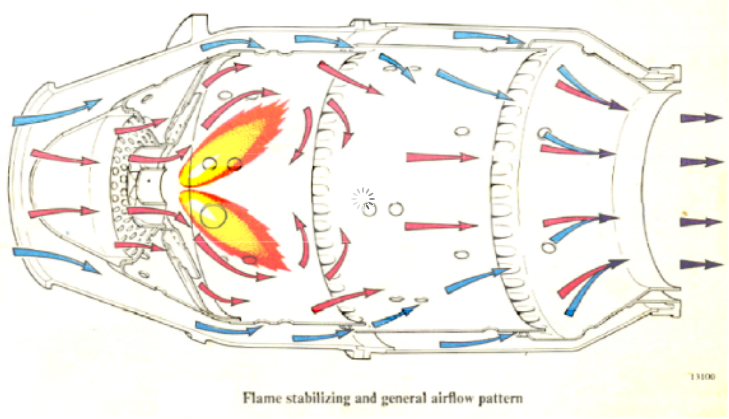
\includegraphics[width=\linewidth]{3.png}
		\caption{Flame stabilization.}
	\end{subfigure}
	\begin{subfigure}[b]{0.49\linewidth}
		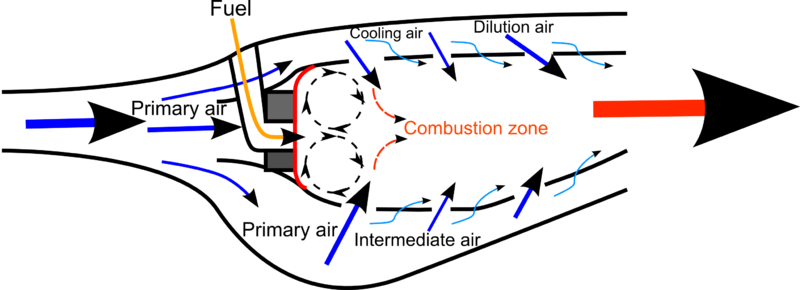
\includegraphics[width=\linewidth]{4.png}
		\caption{Airflow paths in a gas turbine combustor.}
	\end{subfigure}
	\caption{Overall distribution of air through the combustion chamber.}
\end{figure}

As seen in figure 3b, the primary flow of air divides into different sections, it can go to the flare where it will enter directly into the flame casing. It can also differentiate as intermediate air, where it will function as cooling air, isolating the falme casing from the rest of the system, lowering its overall temperature. And this intermidiate air can go into the dilution holes, where it will enter the flame casing in a turbulent manner, mixing with the combustion gases, doping the substance with oxygen.

There are 4 main types of combustors, but in the aerospace industry usually just the first three are the main ones:
\begin{enumerate}
	\item Can Type
	\item Annular Type
	\item Cannular type
	\item Silo type
\end{enumerate}

\subsection*{Can Type}
Also known as tubular type, is one of the older types of combustion chambers. Air leaving the compressor is split into a number of separate streams, each supplying a different chamber. These chambers are spaced around the shaft connecting the compressor and turbine, each chamber having its own fuel jet fed from a common supply line. This desing is well suited for centrifugal compressors, where the flow is divided into separate streams in the diffuser.
\begin{figure}[H]
	\centering
	\begin{subfigure}[b]{0.49\linewidth}
		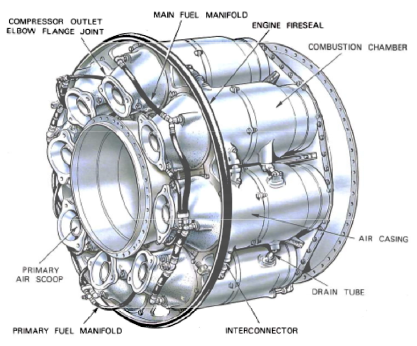
\includegraphics[width=\linewidth]{can.png}
		\caption{Layout of the chambers.}
	\end{subfigure}
	\begin{subfigure}[b]{0.49\linewidth}
		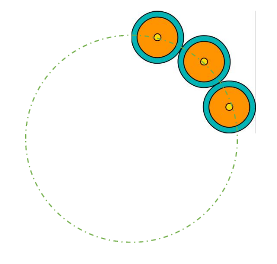
\includegraphics[width=\linewidth]{bcan.png}
		\caption{Cross section of the arrangements of the combustors in the system.}
	\end{subfigure}
	\caption{Can type combustor.}
\end{figure}

\subsection*{Annular Type}
The ideal configuration in terms of compact dimensions is the anular combustor, in which maximum use is made of the space available within a specified diameter; this should reduce the pressure loss and results in an engine of minimum diameter. The combustion does not take place in individual flame tubes,but instead in an annular region around the engine.

It overcomes certain disadvantages the can type combustor has, some of which are the reduction of pressure loss and the compact size it has. Although the annular type comes with its own disavantages. For example, it has less structural integrity, it's difficult to obtain an even temperature distribution and the development/mantainance is difficult overall.

\begin{figure}[H]
	\centering
	\begin{subfigure}[b]{0.49\linewidth}
		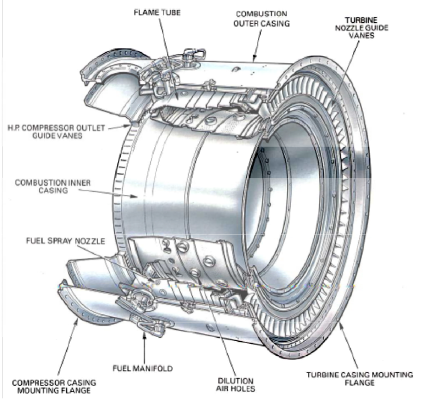
\includegraphics[width=\linewidth]{an.png}
		\caption{General view of the whole chamber.}
	\end{subfigure}
	\begin{subfigure}[b]{0.49\linewidth}
		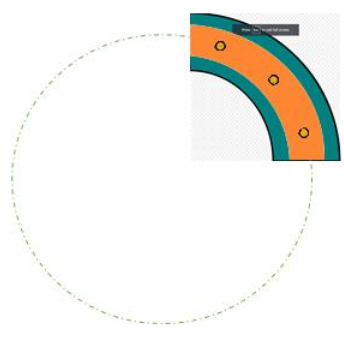
\includegraphics[width=\linewidth]{banu.png}
		\caption{Cross section of the combustors in the system.}
	\end{subfigure}
	\caption{Annular type combustor.}
\end{figure}

\subsection*{Cannular Type}
Also known as tubo-annular type, uses individual flame tubes that are uniformly spaced around an annular casing. Uses a reverse flow arrangemente which allows a significant reduction in the overall length of the compressor-turbine shaft and also permits easy access to the fuel nozzles and combustion cans for maintainance.\autocite{rset}

\begin{figure}[H]
	\centering
	\begin{subfigure}[b]{0.49\linewidth}
		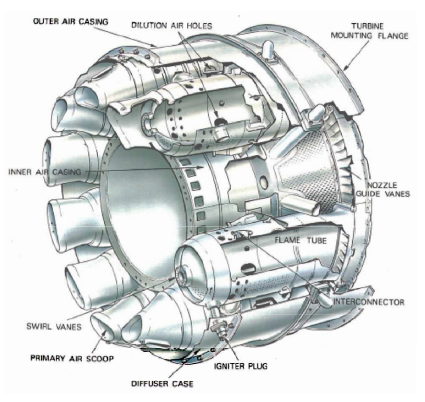
\includegraphics[width=\linewidth]{canular.png}
		\caption{General view of the whole chamber and the arrangement.}
	\end{subfigure}
	\begin{subfigure}[b]{0.49\linewidth}
		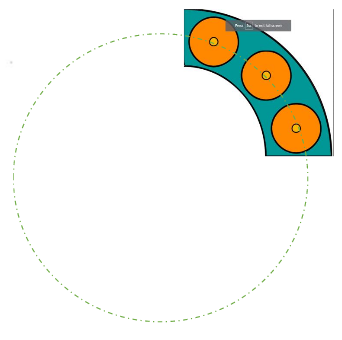
\includegraphics[width=\linewidth]{bcanu.png}
		\caption{Cross section of the combustors in the system.}
	\end{subfigure}
	\caption{Cannular type combustor.}
\end{figure}
%%%%%  Bib
\renewcommand\refname{References}
\printbibliography
\end{document}
